\begin{frame}
\begin{center}
\textbf{
\Huge
CS2105\\[10pt]
	}
\large
An Awesome Introduction to\\ Computer Networking
\end{center}
\end{frame}


\begin{frame}
\begin{center}
\large
Ooi Wei Tsang\\
AS6 05-14\\
\large
\texttt{ooiwt@comp.nus.edu.sg}\\
\end{center}
\end{frame}

\begin{frame}
\begin{center}
\large
Office Hour\\
\large
Monday 4-6pm
\end{center}
\end{frame}

%\begin{frame}
%\begin{center}
%\large
%Your friendly TA\\
%\large
%Loke Yan Hao\\
%\large
%\texttt{Loke.Yan.Hao@gmail.com}\\
%\end{center}
%\end{frame}

\begin{frame}
\begin{center}
	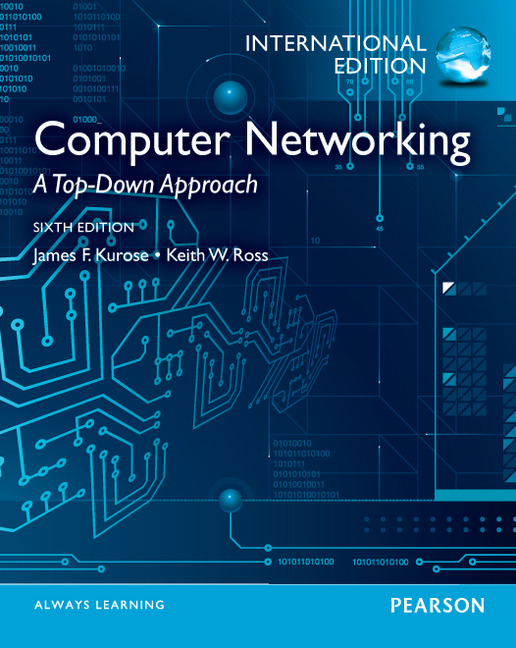
\includegraphics[scale=0.3]{figures/textbook-cover.jpg}
\end{center}
\end{frame}

\begin{frame}
\begin{center}
	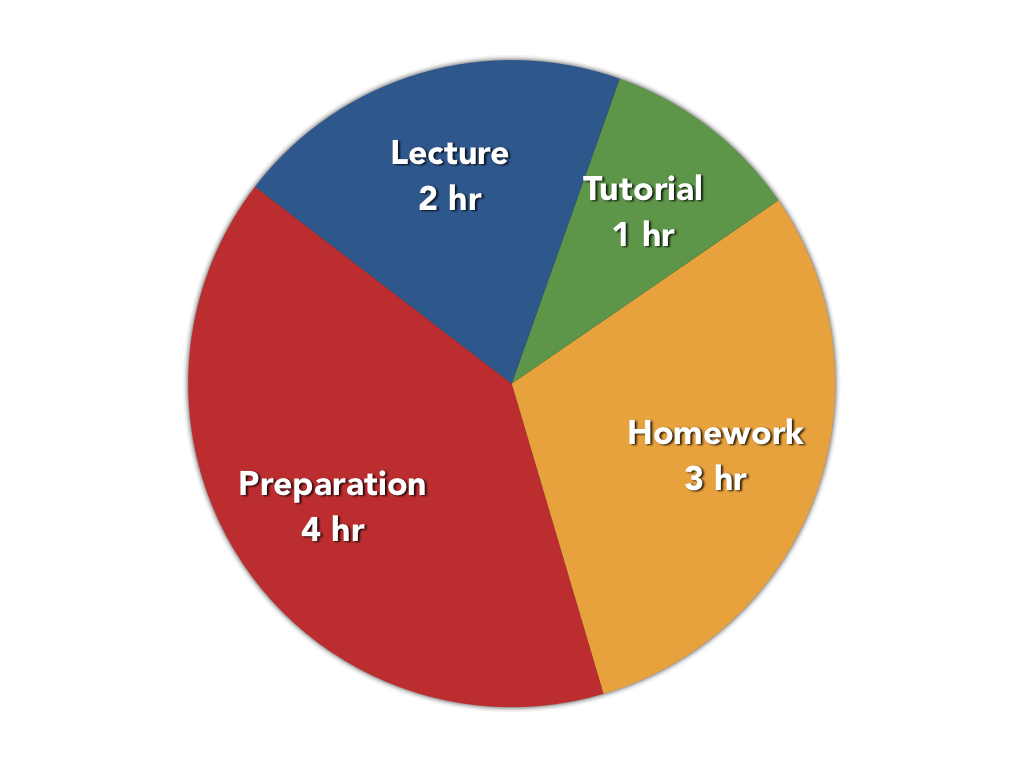
\includegraphics[scale=0.3]{figures/workload-chart.png}
\end{center}
\end{frame}

\begin{frame}
\begin{center}
	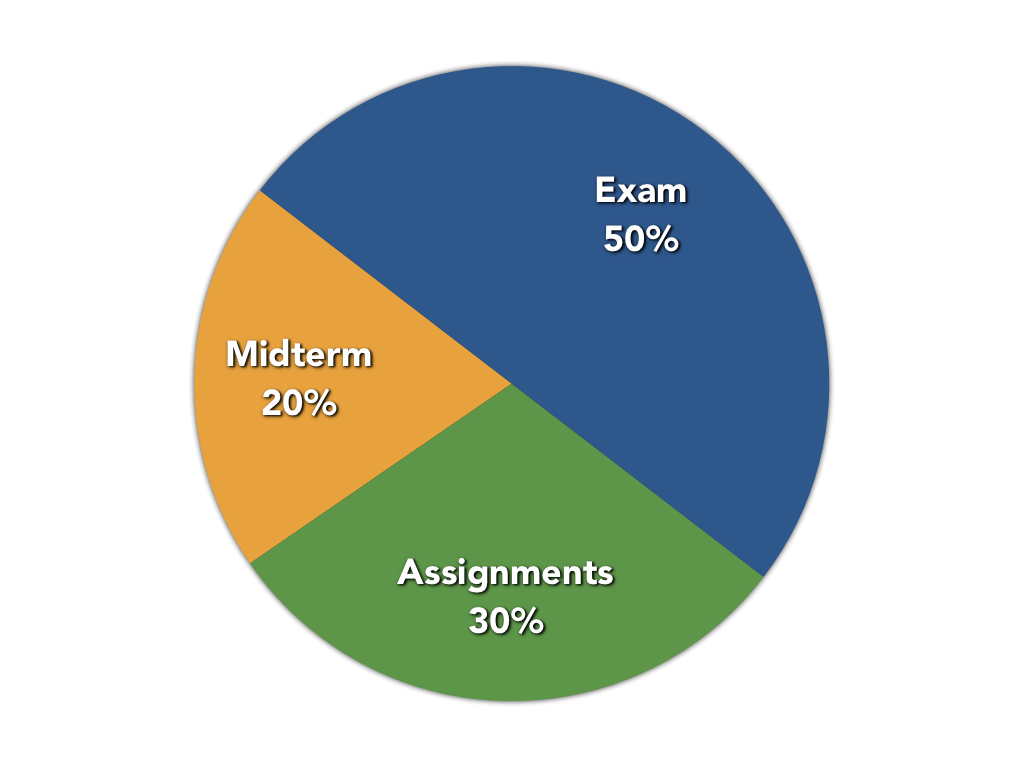
\includegraphics[scale=0.3]{figures/assessment-chart.png}
\end{center}
\end{frame}

\begin{frame}
\begin{center}
\large
2 programming assignments\\
1 written assignment\\
9 problem sets\\
4 practical exercises\\
\end{center}
\end{frame}

\begin{frame}
\begin{center}
\large
Important Dates\\
Midterm: \textbf{10 March 2014}\\
Final Exam: \textbf{30 April 2014}
\end{center}
\end{frame}

\begin{frame}
\begin{center}
\large
Midterm \& Final are\\
\large
\textbf{Semi-Open Book}\\
\normalsize
(one double-sided A4 crib sheet allowed)
\end{center}
\end{frame}

\begin{frame}
\begin{center}
\large
Slides to be posted 1-2 days before lecture
\end{center}
\end{frame}

\begin{frame}
\begin{center}
\large
Slides $\not=$ Notes
\end{center}
\end{frame}

\begin{frame}
\begin{center}
\large
You are expected to \textbf{take notes} during lecture
\end{center}
\end{frame}

\begin{frame}
\begin{center}
\large
You are expected to \textbf{read} the assigned readings
\end{center}
\end{frame}

\begin{frame}
\begin{center}
\large
No model answer will be posted
\end{center}
\end{frame}

{% all template changes are local to this group.
\setbeamertemplate{navigation symbols}{}
\begin{frame}[plain]
\begin{tikzpicture}[remember picture,overlay]
	\node[at=(current page.center)] {
		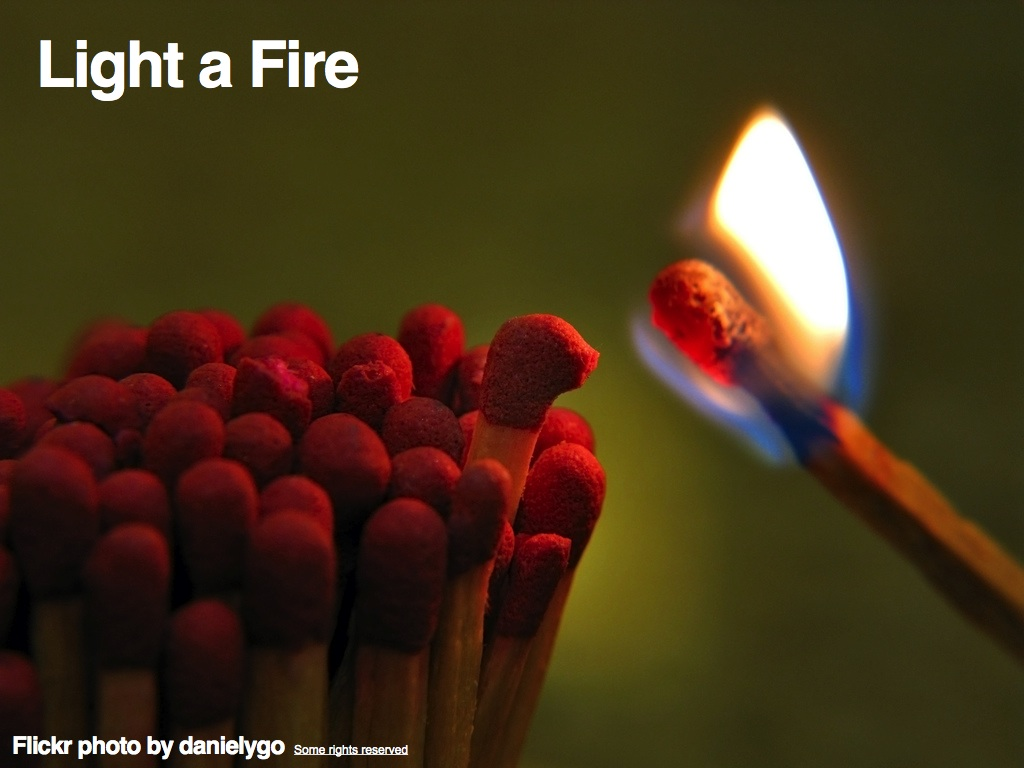
\includegraphics[width=\paperwidth]{figures/light-a-fire.jpg}
	}; 
\end{tikzpicture}
\end{frame}

\begin{frame}[plain]
\begin{tikzpicture}[remember picture,overlay]
	\node[at=(current page.center)] {
		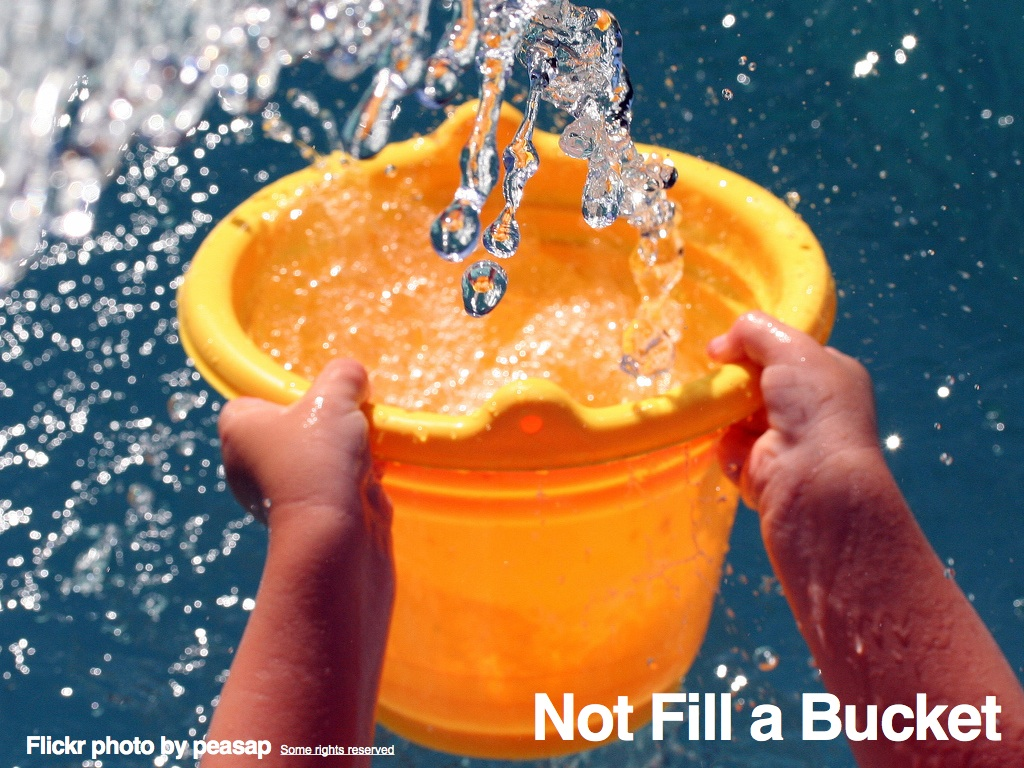
\includegraphics[width=\paperwidth]{figures/fill-a-bucket.jpg}
	}; 
\end{tikzpicture}
\end{frame}
}

\begin{frame}
\begin{center}
\large
	\textbf{``No mercy''} policy against\\\textbf{plagiarism}
\end{center}
\end{frame}

\begin{frame}
\begin{center}
\large
	\textbf{``No mercy''} policy against\\voilation of \textbf{naming convention}
\end{center}
\end{frame}

\begin{frame}
\begin{center}
\large
	\url{http://blog.nus.edu.sg/cs2105}
\end{center}
\end{frame}

\begin{frame}
\begin{center}
\large
Check for updates frequently and\\subscribe via email or RSS
\end{center}
\end{frame}

\begin{frame}
\begin{center}
\large Use your real name when comment online
\end{center}
\end{frame}

\begin{frame} \begin{center} \large
Screencast will be posted 
\end{center} \end{frame}

\begin{frame} \begin{center} \large
You need an SoC UNIX account.  Get one here:\\
\url{https://mysoc.nus.edu.sg/~newacct/}
\end{center} \end{frame}

\begin{frame}
\begin{center}
\large
Questions?
\end{center}
\end{frame}

\begin{frame}
\begin{center}
\large
CS2105 Lecture 1\\
\Huge
\textbf{Introduction\\[10pt]}
\normalsize
	14 January, 2014
\note{
\tiny
After this class, you are expected to:
\begin{itemize} 
\item understand the basic terms, including host, packet, protocol, throughput, bottleneck link, store-and-forward, and autonomous system.
\item know about the logical (the five layers) and physical architecture (as a network of ASes) of the Internet.
\item know about the pros and cons of packet switching versus circuit switching.
\item understand the different components of end-to-end delay and their relations to bandwidth, packet size, distance, propagation speed, and queue size.
\end{itemize} 
}
\end{center}
\end{frame}

\begin{frame}
\begin{center}
\large
Lecture 1\\
\normalsize
You won't believe how complex the Internet is.  But once you see the simple trick used to keep the complexity manageable, you will go.. Wow!
\end{center}
\end{frame}

\begin{frame}
\begin{center}
\large
What is
\large
CS2105\\
\large
about?
\end{center}
\end{frame}

\begin{frame}
\begin{center}
\large
\textbf{Concepts} and \textbf{principles}\\
behind computer networking\\[20pt]
\large
Introduction to networked application programming\\
\end{center}
\end{frame}

\begin{frame}
\begin{center}
\large
\textbf{The Internet} is a network of connected computing devices.
\end{center}
\end{frame}

\begin{frame}[plain]\begin{center}\large
		\textbf{Hosts} or \textbf{end systems} \\
		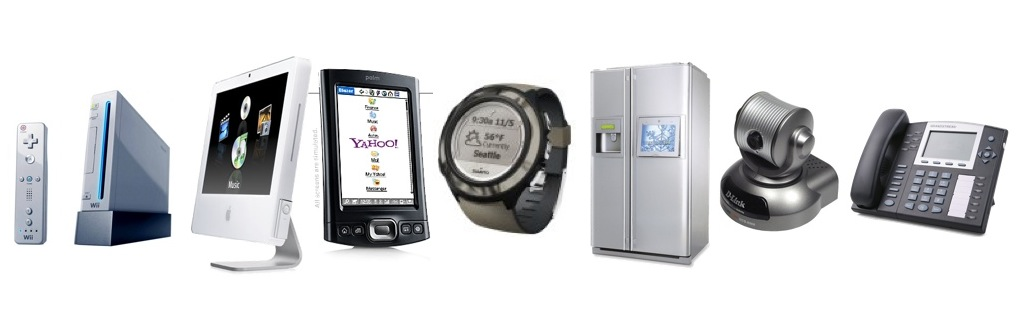
\includegraphics[width=\linewidth]{figures/end-host-examples.jpg}
\end{center}\end{frame}

\begin{frame}[plain]\begin{center}\large
		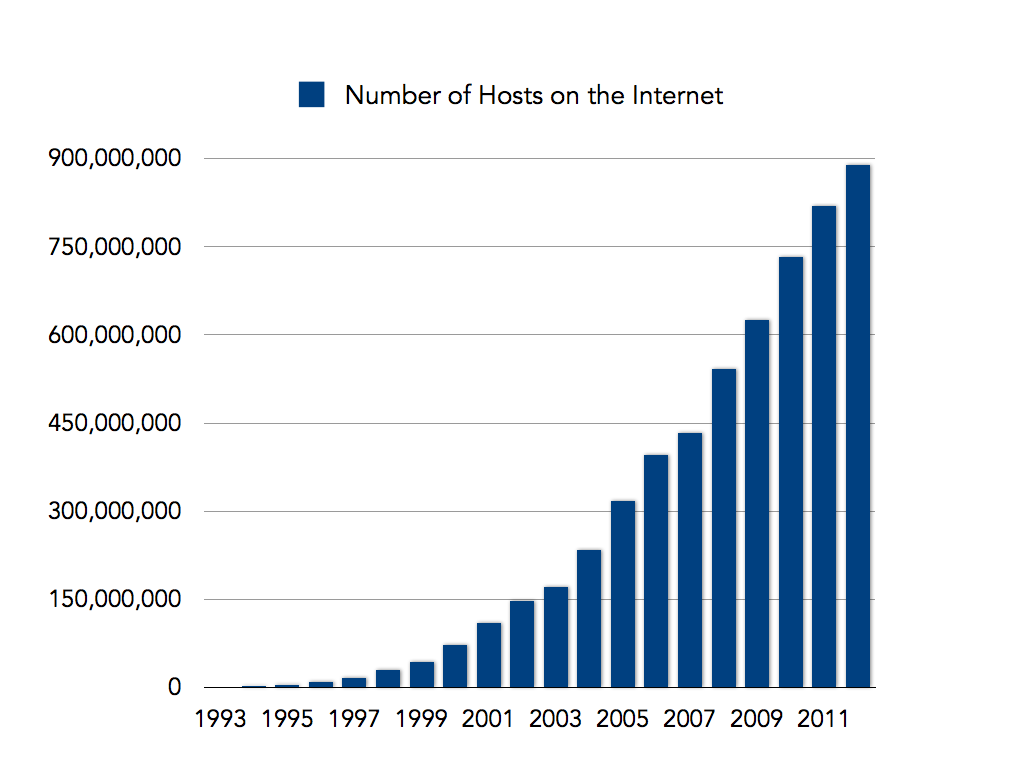
\includegraphics[width=\linewidth]{figures/num-of-hosts-chart.png}
\end{center}\end{frame}

\begin{frame}
\begin{center}
\Huge
\textbf{996,230,757}\\
\large
as of July 2013
\note{
Data obtained from Internet Systems Consortium: 
\url{http://www.isc.org/solutions/survey/history}
}
\end{center}
\end{frame}

\begin{frame}\begin{center}
\large
The hosts run \textbf{distributed applications}
\end{center}\end{frame}

\begin{frame}
\large
\textbf{Web}: browsers, Web servers\\
\textbf{WoW}: clients, game servers\\
\textbf{Skype}: clients, supernodes\\
\textbf{BitTorrent}: peers, trackers\\
\end{frame}

\begin{frame}
\begin{center}
\large
Applications\\\textbf{exchange messages} and\\ communicate according to \textbf{protocols}
\end{center}
\end{frame}

\begin{frame}
\begin{center}
\large
\textbf{Protocol:} the \textbf{type} and \textbf{order} of messages exchanged and the \textbf{actions} taken after messages are sent or received
\end{center}
\end{frame}

\begin{frame}
\begin{center}
\large
Examples:\\
\textbf{HTTP, SMTP, FTP, TCP}
\end{center}
\end{frame}

\begin{frame}
\begin{center}
\large
The hosts access the Internet through \textbf{access network}
\end{center}
\end{frame}

\begin{frame}\begin{center}
\large
WiFi, Ethernet, 3G, LTE, DSL, Cable, Fiber, Dial-Up, Satellite
\note{
You can read up more about these different access network technologies in Section 1.2.1.  We will cover Ethernet and WiFi in more details in CS2105. 
}
\end{center}\end{frame}

\begin{frame}
\begin{center}
\large
Hosts can communicate over different \textbf{physical media}
\end{center}
\end{frame}

\begin{frame}[plain]\begin{center}
\begin{tikzpicture}[remember picture,overlay]
	\node[at=(current page.center)] {
		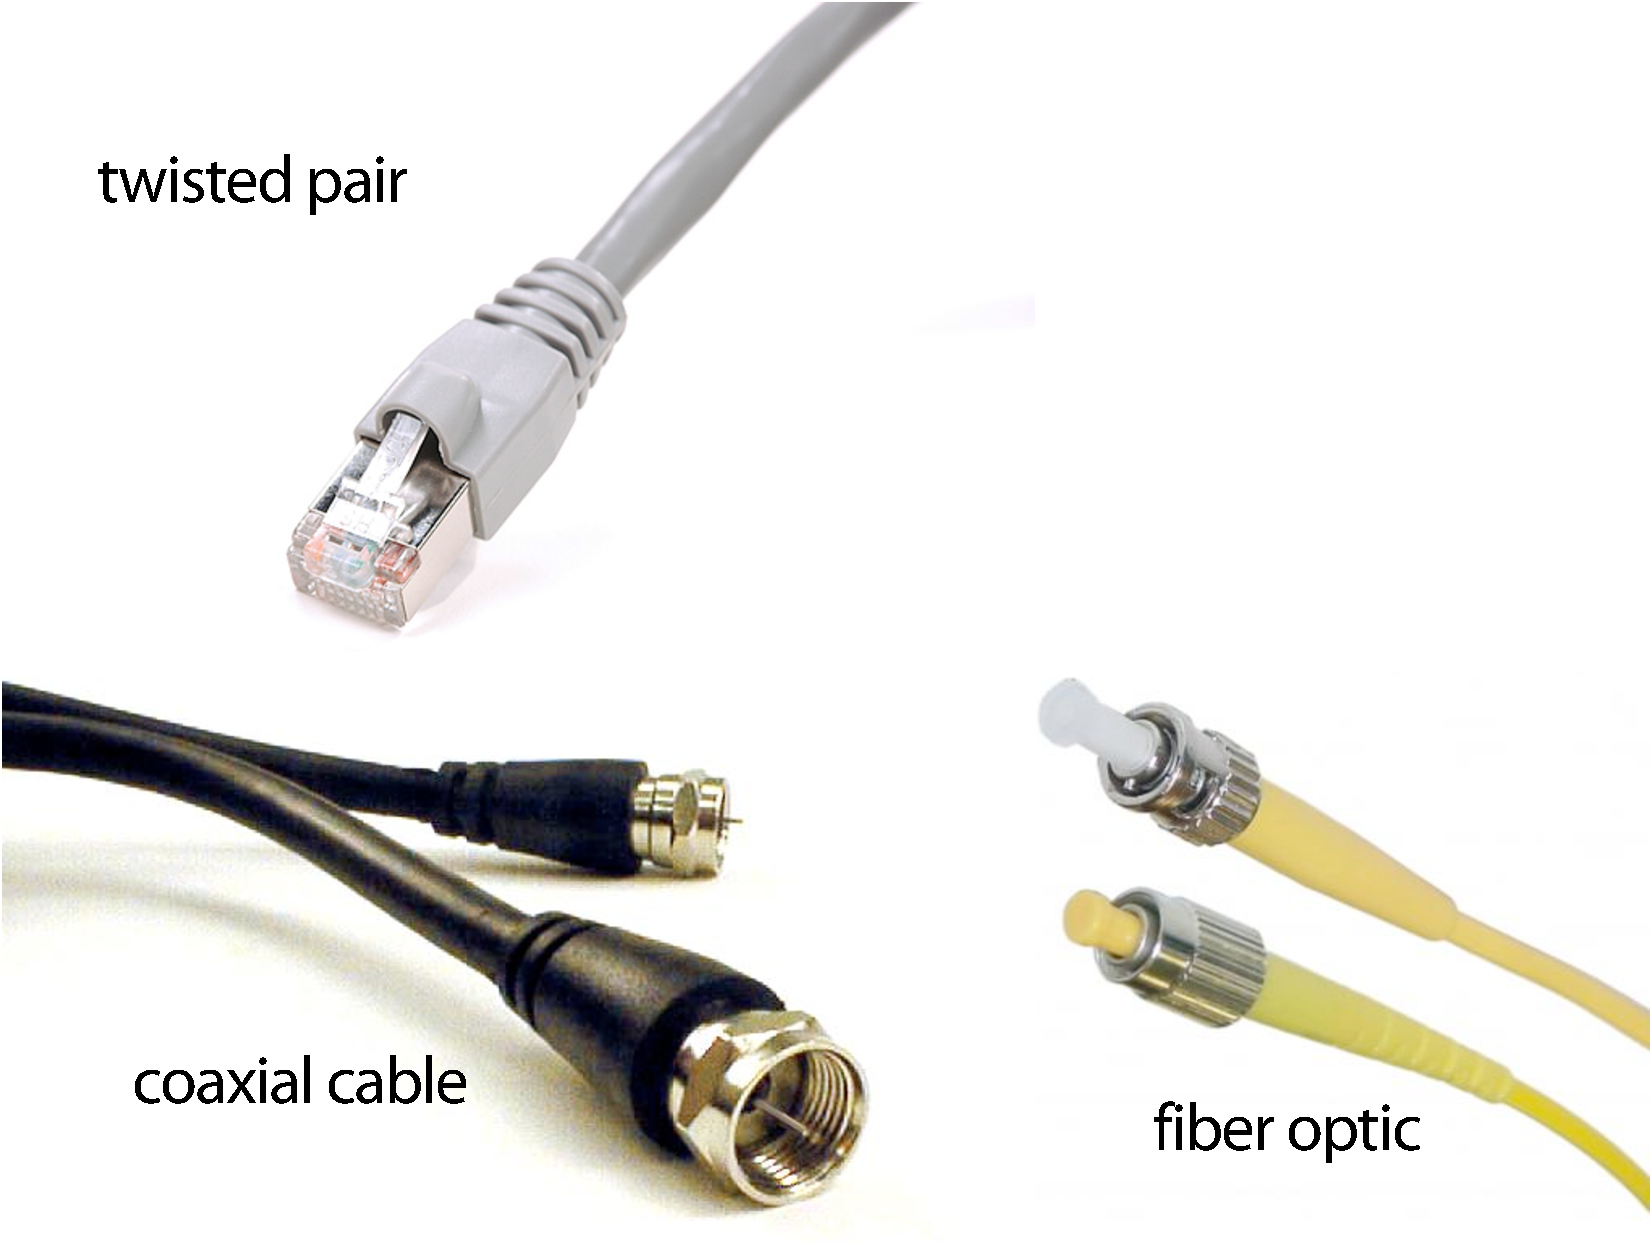
\includegraphics[width=\paperwidth]{figures/physical-media-crop.pdf}
	}; 
\end{tikzpicture}
\end{center}\end{frame}

\begin{frame}[t]\normalsize
	Consider two hosts connected directly through a physical medium
\end{frame}

\begin{frame}[t]\normalsize
	The hosts communicate by sending information to each other.
\end{frame}

\begin{frame}[t]\normalsize
	Information can be represented with a sequence of bits -- 0 or 1.
\end{frame}

\begin{frame} \begin{center} \large
	\textbf{Modulation/Demodulation}:\\ Conversion between bits and signals\\
\end{center} \end{frame}

\begin{frame} \begin{center} \large
	\textbf{Error Detection/Correction}:\\ Ensuring that bits are received correctly\\
\end{center} \end{frame}

\begin{frame}\begin{center}\large
	\textbf{Packetization/Segmentation}:\\ \large Dividing data into chunks (called \textit{packets}) 
	so that only errornous packets need to be retransmitted.
\end{center}\end{frame}

\begin{frame}[t]\normalsize
	Consider multiple hosts connected through a shared physical medium
\end{frame}

\begin{frame}\begin{center}\large
	\textbf{Addressing}:\\ Identify the source and destination
\end{center}\end{frame}

\begin{frame}\begin{center}\large
	\textbf{Medium access control}:\\ Regulate who sends
\end{center}\end{frame}

\begin{frame}[t]\normalsize
	Consider multiple hosts connected through \textbf{intermediate packet switches}, 
	which \textbf{store and forward} the packets.
\end{frame}

\begin{frame}[plain]\begin{center}
\begin{tikzpicture}[remember picture,overlay]
	\node[at=(current page.center)] {
		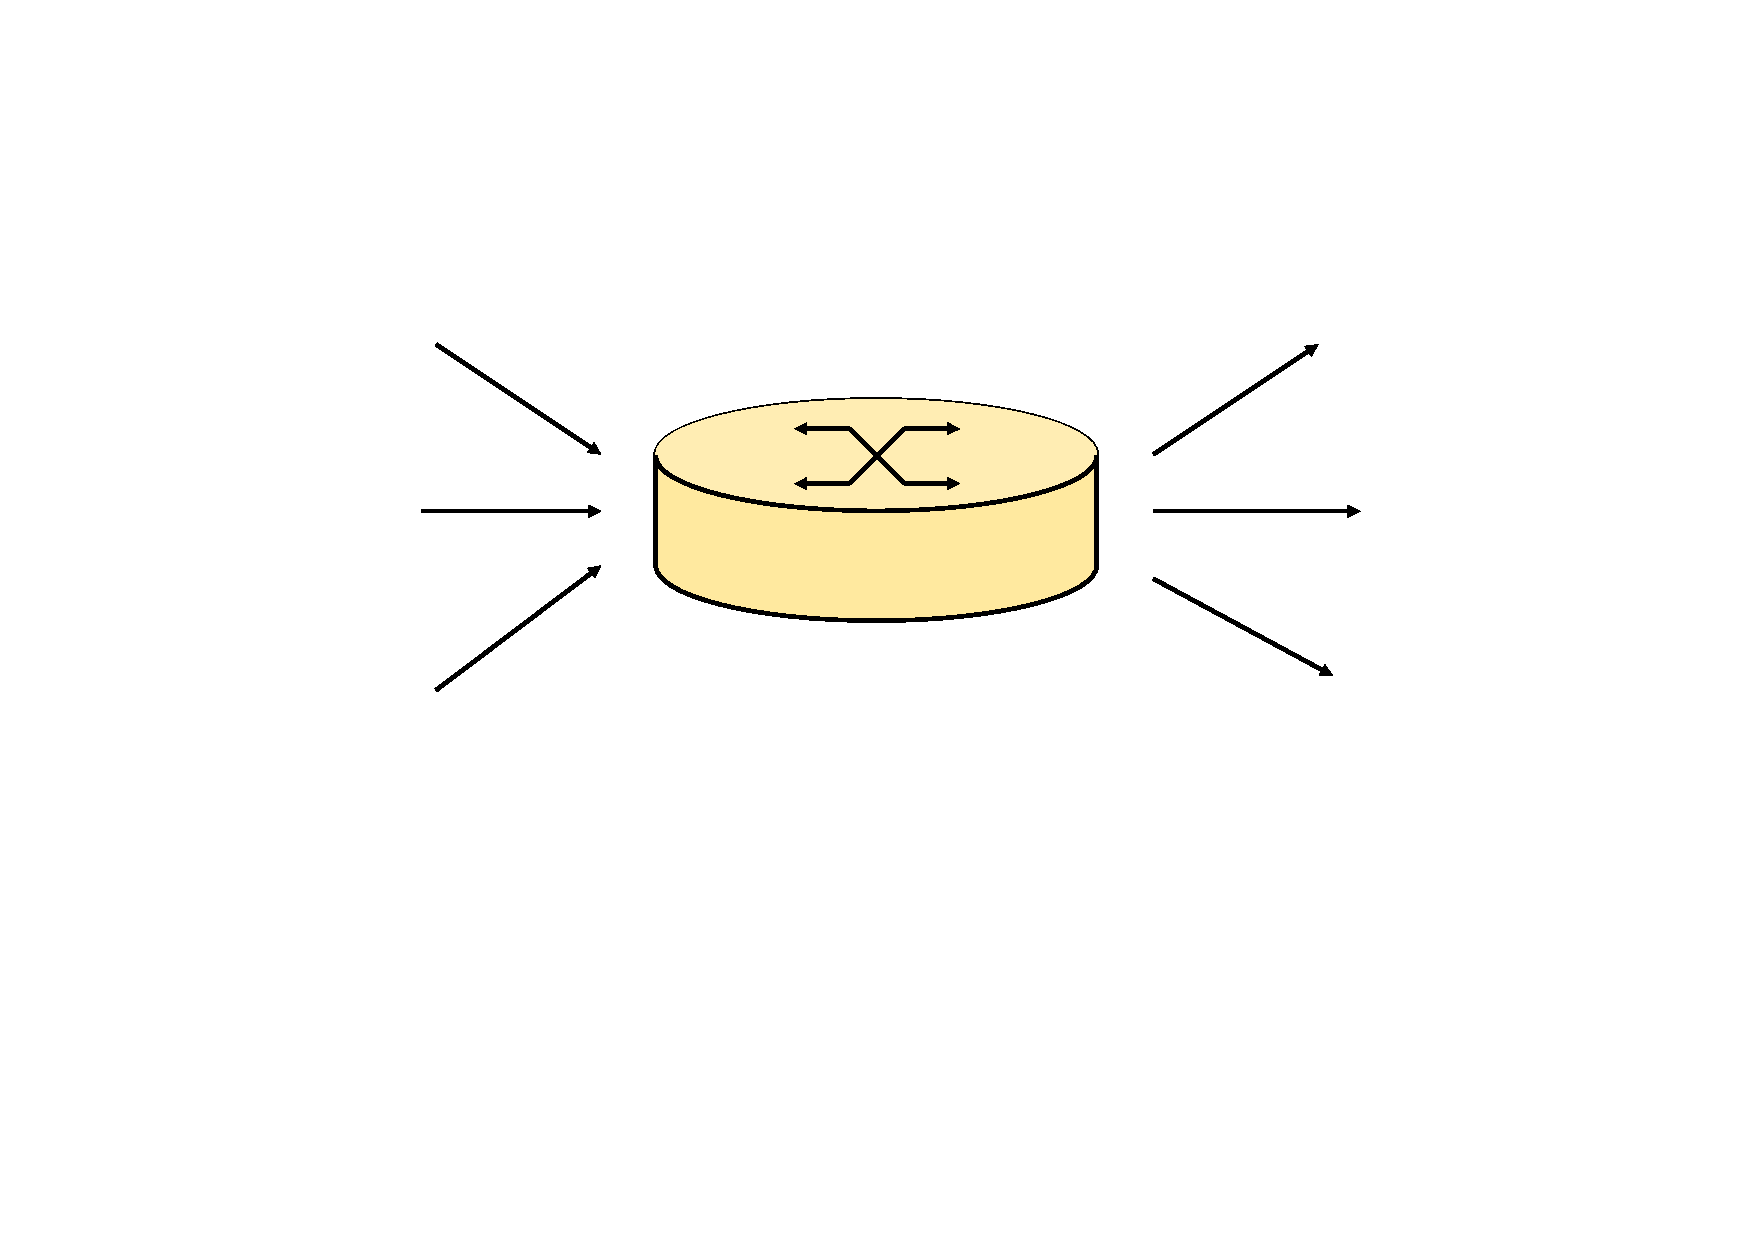
\includegraphics[width=\paperwidth]{figures/store-and-forward.pdf}
	}; 
\end{tikzpicture}
\end{center}\end{frame}

\begin{frame}\begin{center}\large
The Internet is a \textbf{packet switching} network
\end{center}\end{frame}

\begin{frame}\begin{center}\large
\textbf{Packet switching}:\\\large Resources used on demand;\\best effort services
\end{center}\end{frame}

\begin{frame}\begin{center}\large
\textbf{Circuit switching}:\\\large Resources are reserved, guaranteeing services
\end{center}\end{frame}

\begin{frame}\begin{center}\large
\textbf{Packet vs Circuit Switching}:\\\large Which is more efficient?
\note{
	Details about packet switching and circuit switching is explained in Sections 1.3.1 and 1.3.2}
\end{center}\end{frame}

\begin{frame} \begin{center}\large
Who owns the intermediate packet switches on the Internet?
\end{center}\end{frame}

\begin{frame}[plain]\begin{center}
\begin{tikzpicture}[remember picture,overlay]
	\node[at=(current page.center)] {
		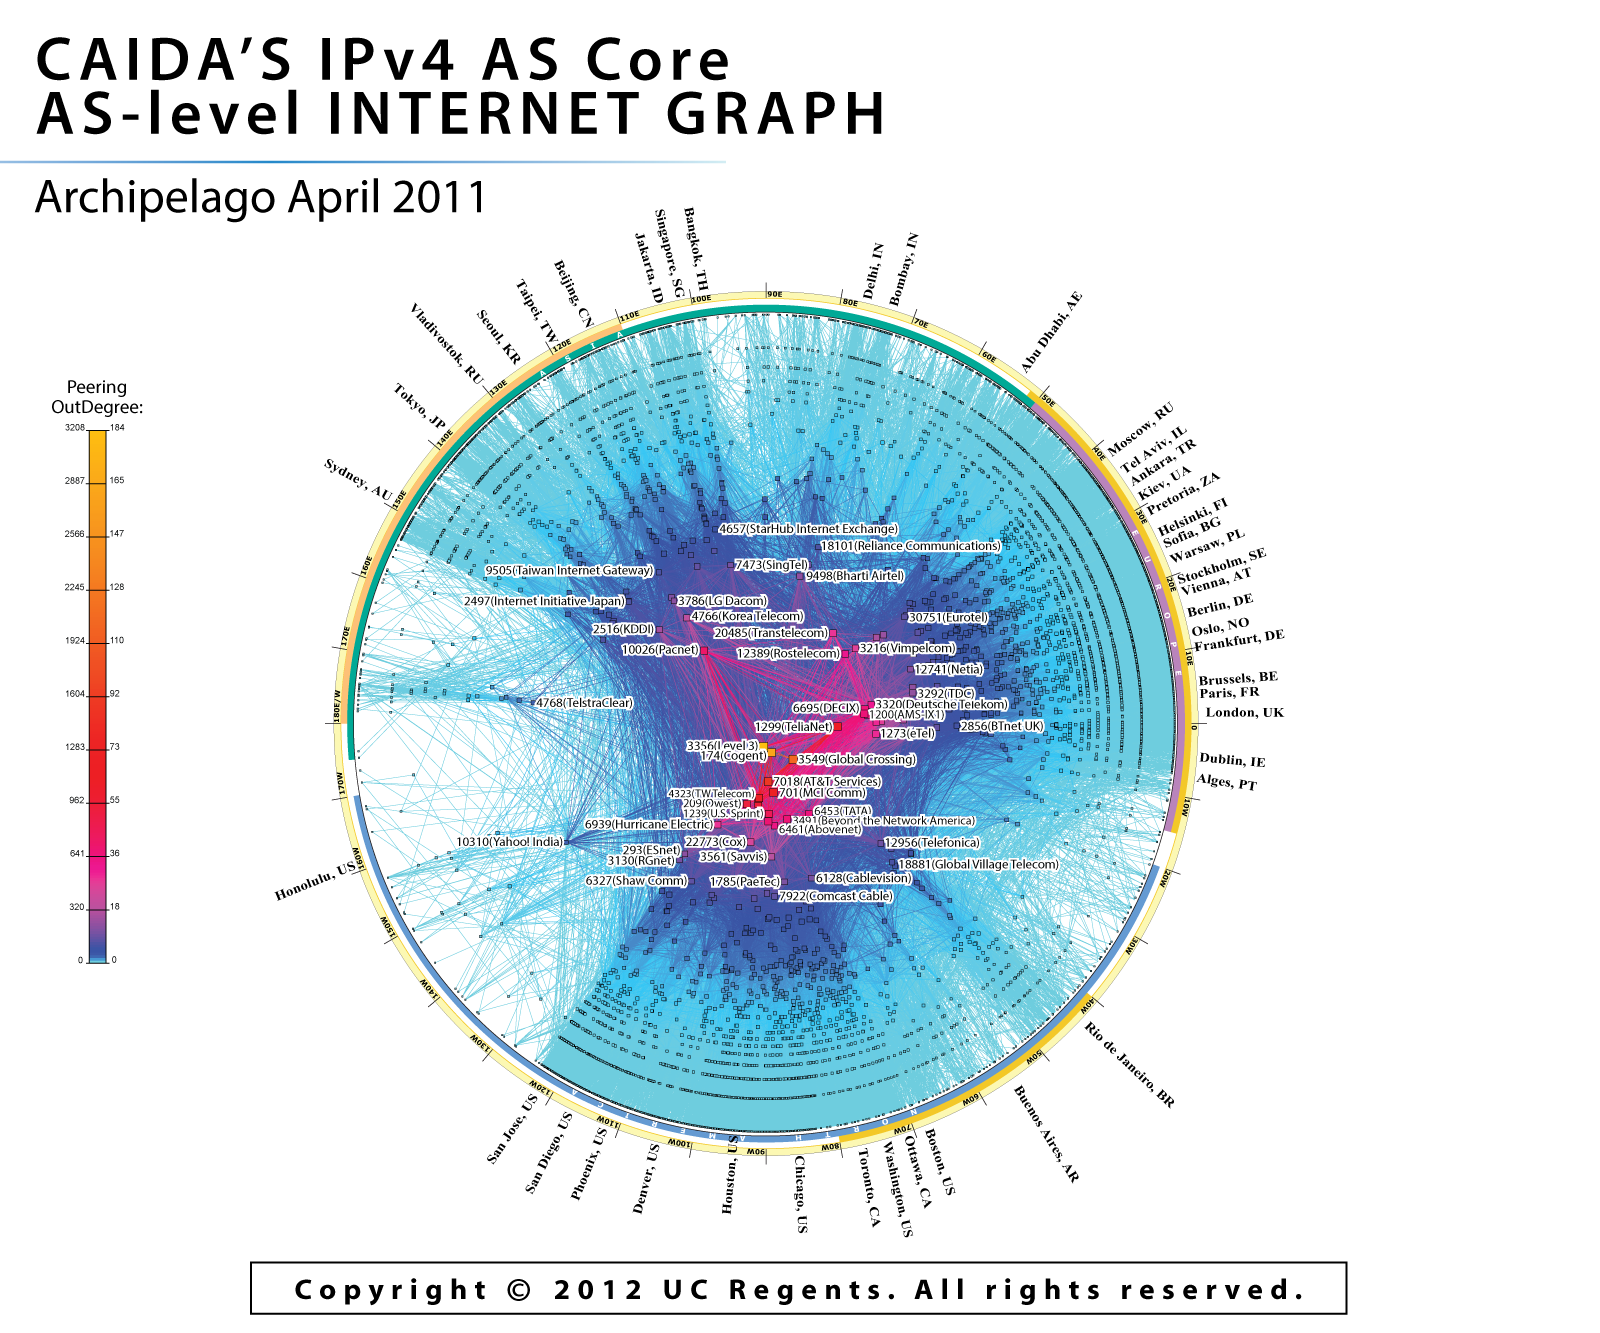
\includegraphics[height=\paperheight]{figures/ascore-2011-apr-ipv4-standalone-1600x1333.png}
	}; 
\end{tikzpicture}
\end{center}\end{frame}

\begin{frame} \begin{center}\large
The Internet is a ``network-of-networks'', organized into autonomous systems (AS), each is owned by an organization.
\note{
To learn more about the architecture of the Internet, read Section 1.3.3.
The Internet topology figure is taken from \url{http://www.caida.org/research/topology/as_core_network/}
}
\end{center}\end{frame}

\begin{frame} \begin{center}\large
\textbf{traceroute}
\note{You can also try to traceroute from other locations on the Internet at \url{http://www.traceroute.org}}
\end{center}\end{frame}

\begin{frame} \begin{center}\large
\textbf{Routing}: Decide which path/route to take
\end{center}\end{frame}

\begin{frame}\begin{center}\large
\textbf{Reliability}: Recover from packet losses
\end{center}\end{frame}

\begin{frame}\begin{center}\large
\textbf{Link Rate}:\\ How many bits can be ``pushed'' onto a link per unit time.
\end{center}\end{frame}

\begin{frame}\begin{center}\large
\textbf{Delay}:\\ Time between send and receive
\end{center}\end{frame}

\begin{frame}\normalsize
To send a packet in a packet switch network, for each link in the path
\begin{enumerate}
\item transmit packet onto link as bits
\item propagate bits to next node
\item store and process the packet
\item wait to be transmitted
\end{enumerate}
\end{frame}

\begin{frame}\normalsize
End-to-end packet delay consists of:
\begin{enumerate}
\item transmission delay
\item propagation delay
\item processing delay
\item queueing delay
\end{enumerate}
\end{frame}

\begin{cf}{
	\begin{tikzpicture}[scale=2]
		\draw[solid] (0,0) -- (0,3);
		\draw[solid] (2,0) -- (2,3);
	\end{tikzpicture}
	}
\end{cf}


\begin{cf}{
\textbf{Throughput}:\\ How many bits can be communicated per unit time.
}
\end{cf}

\begin{frame}[t]\normalsize
	Multiple applications can run on each host
\end{frame}

\begin{cf}{
\textbf{Demultiplexing}: Determine which packet belongs to which application
}
\end{cf}

\begin{frame}\begin{center}\normalsize
Many issues to consider, to support different applications running on large number of hosts through different access technology and physical media.
\end{center}\end{frame}

\begin{frame}[plain]
\begin{tikzpicture}[remember picture,overlay]
	\node[at=(current page.center)] {
		
\includegraphics[width=\paperwidth]{figures/confused-jackie.jpg}
	}; 
\end{tikzpicture}
\end{frame}

\begin{frame}\begin{center}\large
\textbf{Layering}:\\Common CS trick to deal with large and complex systems
\end{center}\end{frame}

\begin{frame}\begin{center}\large
Each layer provides a service;\\ Simple interfaces btwn layers;\\ Hide details from each other.
\note{
	The five layers of the Internet is described in Section 1.5.}
\end{center}\end{frame}

%\begin{frame}[plain]
%\begin{tikzpicture}[remember picture,overlay]
%	\node[at=(current page.center)] {
%		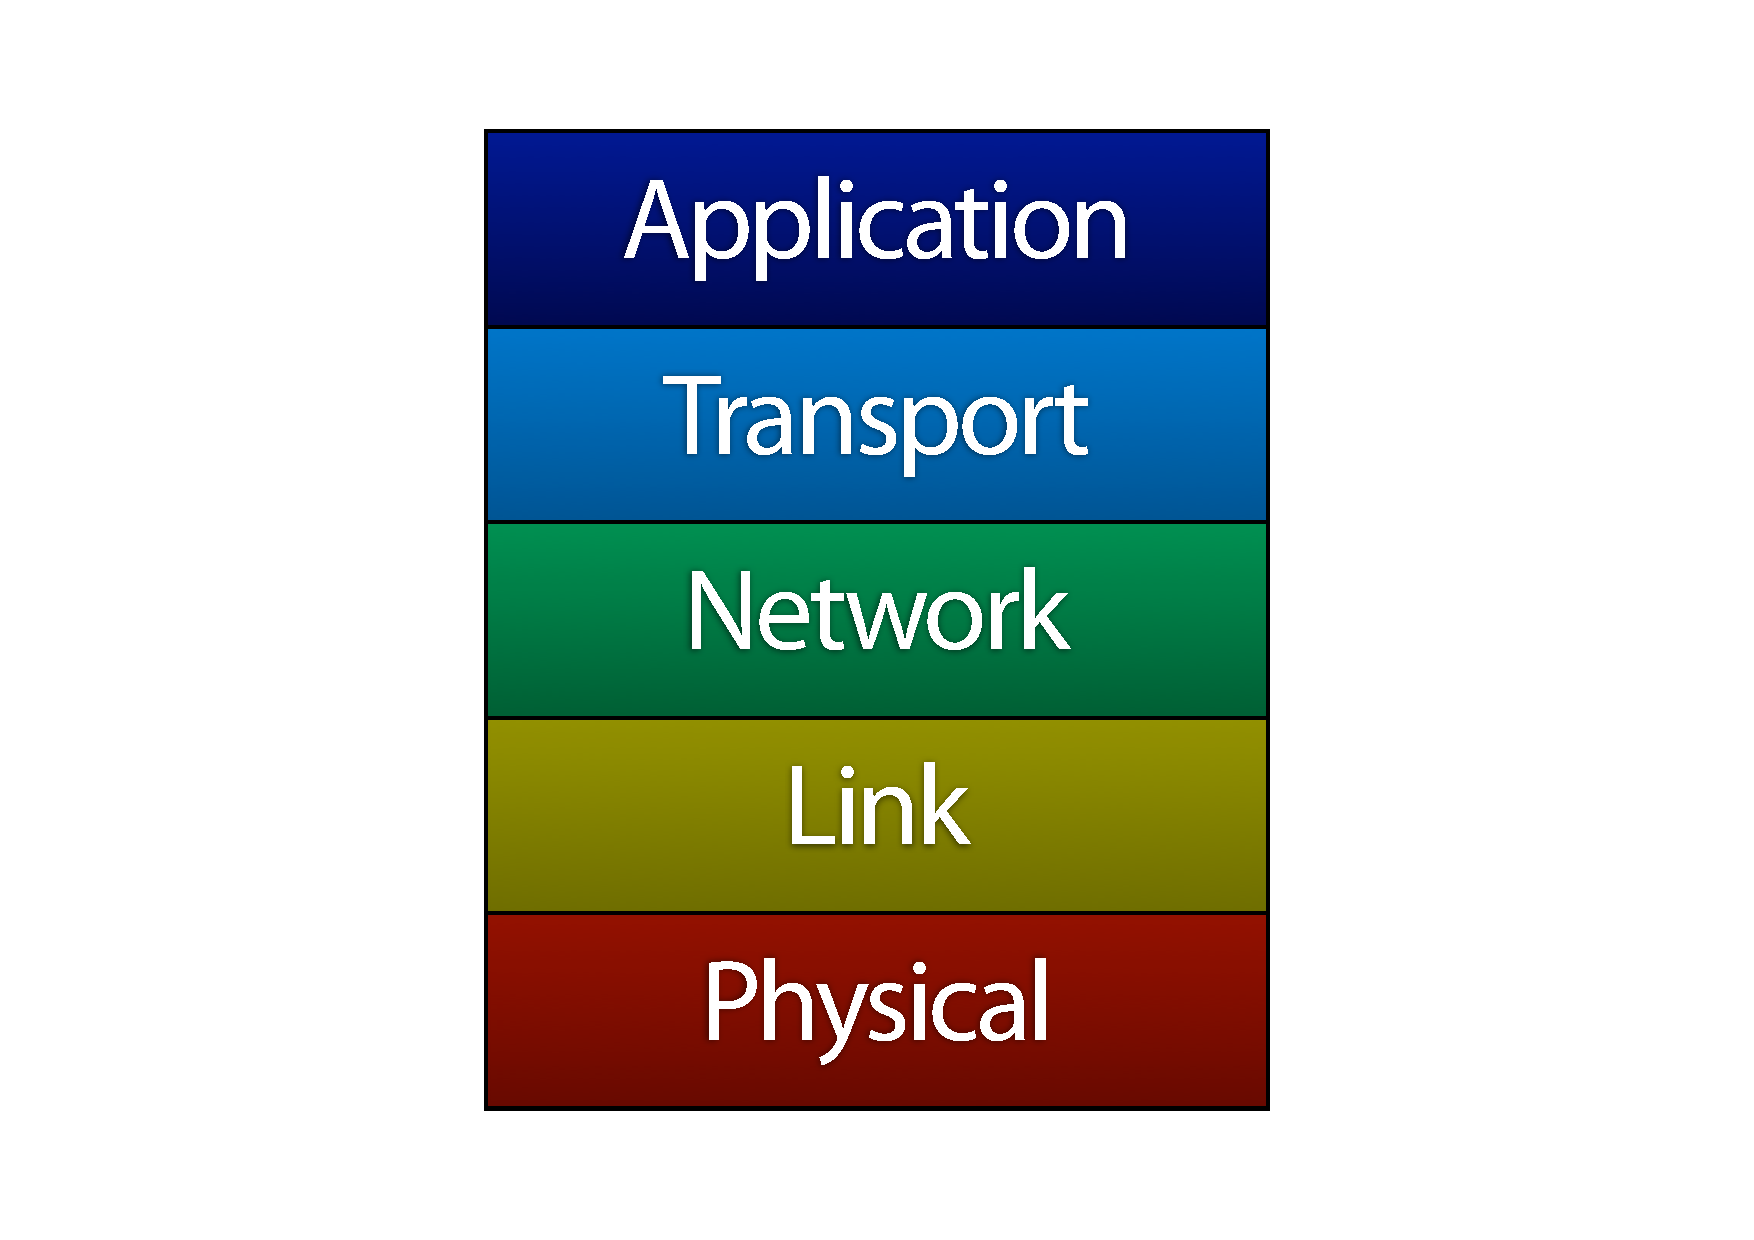
\includegraphics[width=\paperwidth]{figures/layers.pdf}
%	}; 
%\end{tikzpicture}
%\end{frame}

\begin{frame}
\begin{center}
\tikzstyle{layer}=[draw,rectangle,minimum height=1.5 cm, minimum width=5 cm, text=white]
	\begin{tikzpicture}[scale=2]
	\node[layer](A)[fill=AppBlue]{Application};
	\node[layer](T)[below = 0cm of A,fill=TransportBlue]{Transport};
	\node[layer](N)[below = 0cm of T,fill=NetworkGreen]{Network};
	\node[layer](L)[below = 0cm of N,fill=LinkBrown]{Link};
	\node[layer](P)[below = 0cm of L,fill=PhysicalRed]{Physical};
	\end{tikzpicture}
\end{center}
\end{frame}

\begin{frame}\begin{center}\large
Applications (or processes) treat the Internet as a \textbf{black box}, sending and receiving messages through a \textbf{socket}.
\end{center}\end{frame}

\begin{frame}\begin{center}\large
\textbf{Transport layer}\\\large provides process-to-process message delivery services.
\end{center}\end{frame}

\begin{frame}\begin{center}\large
\textbf{TCP}\\
\large reliable, in-order delivery, with congestion and flow control
\end{center}\end{frame}

\begin{frame}\begin{center}\large
\textbf{UDP}\\
\large best-effort delivery
\end{center}\end{frame}

\begin{frame}\begin{center}\large
\textbf{Network layer}\\ 
\large host-to-host delivery 
\end{center}\end{frame}

\begin{frame}\begin{center}\large\textbf{Link layer}\\ 
\large node-to-node delivery 
\end{center}\end{frame}

\begin{frame}\begin{center}\large
\textbf{Physical layer}\\\large ``bits over physical media'' 
\end{center}\end{frame}
